\chapter{Введение}

\section{Цель работы}

Знакомство с системой защиты информации от несанкционированного доступа Dallas Lock 8.0


\chapter{Ход работы}

\begin{figure}[H]
	\centering
	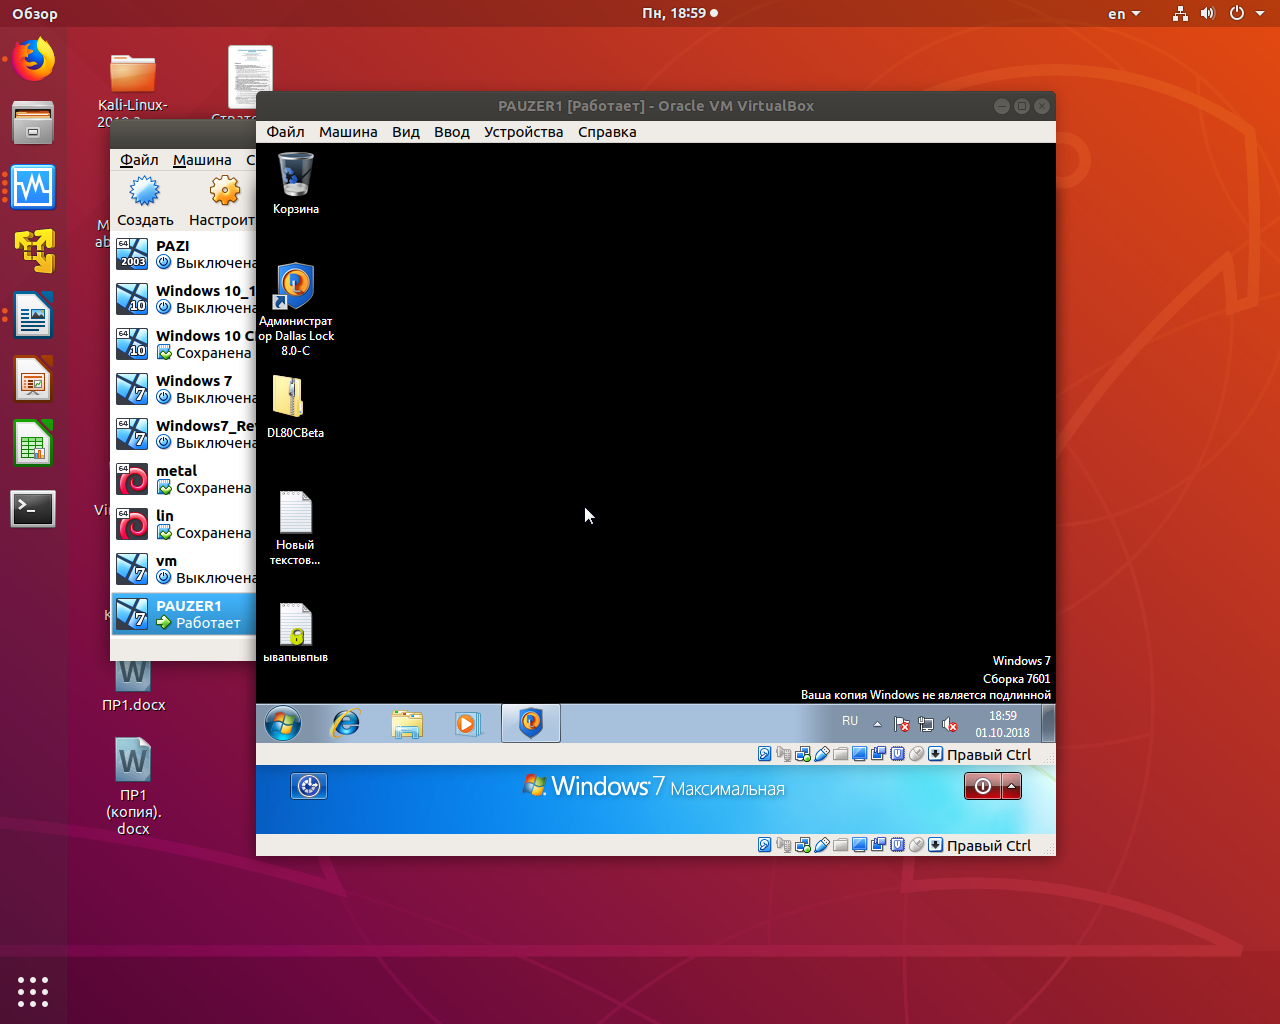
\includegraphics[width=.8\textwidth]{images/1.png}
	\caption{Вход в виртуальную машину}
\end{figure}

\begin{figure}[H]
	\centering
	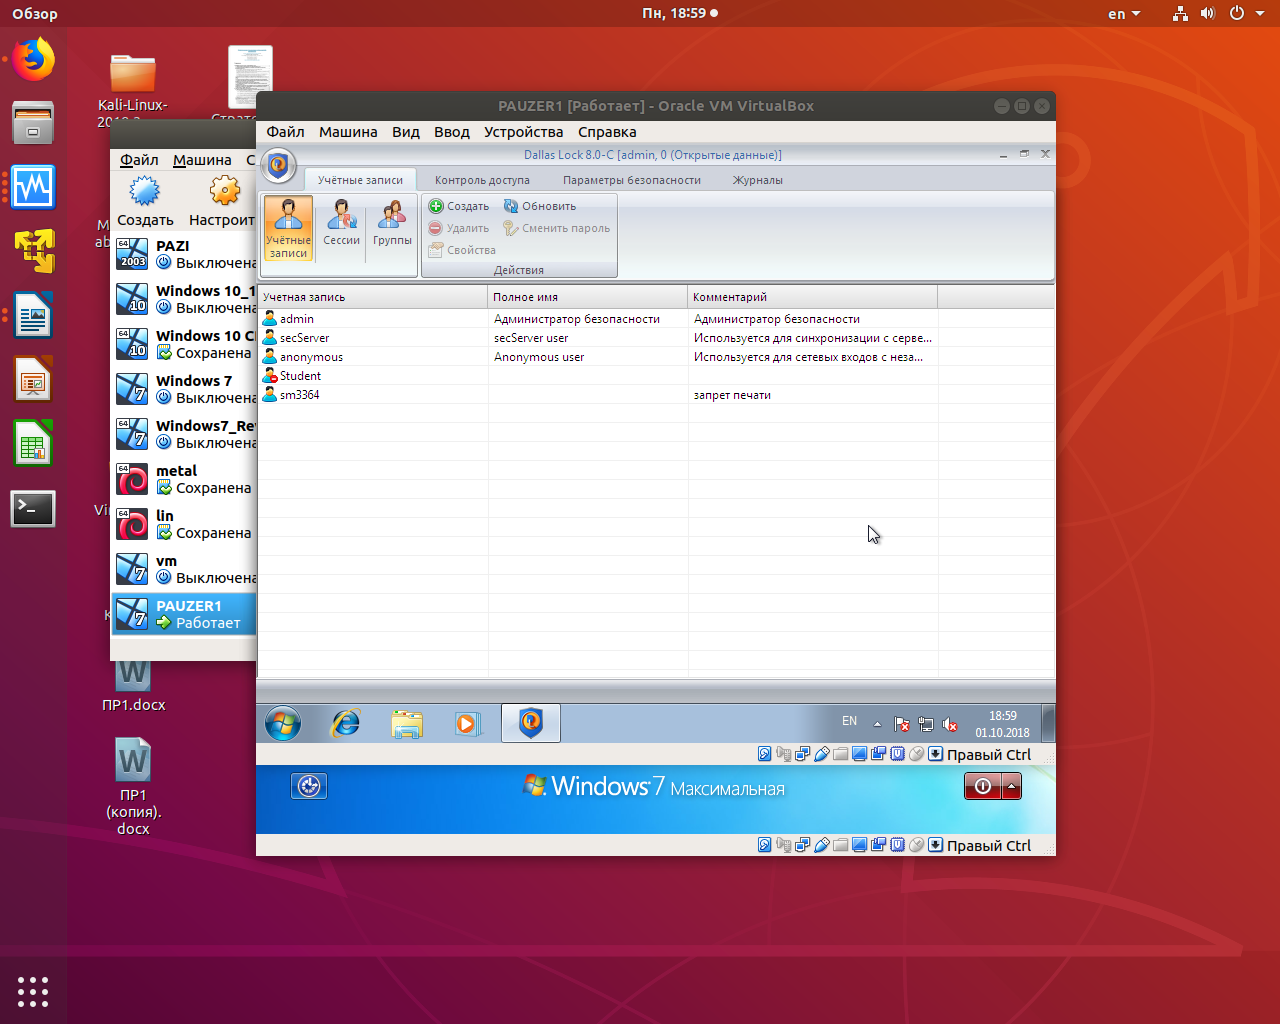
\includegraphics[width=.8\textwidth]{images/2.png}
	\caption{Запрет печати}
\end{figure}

\begin{figure}[H]
	\centering
	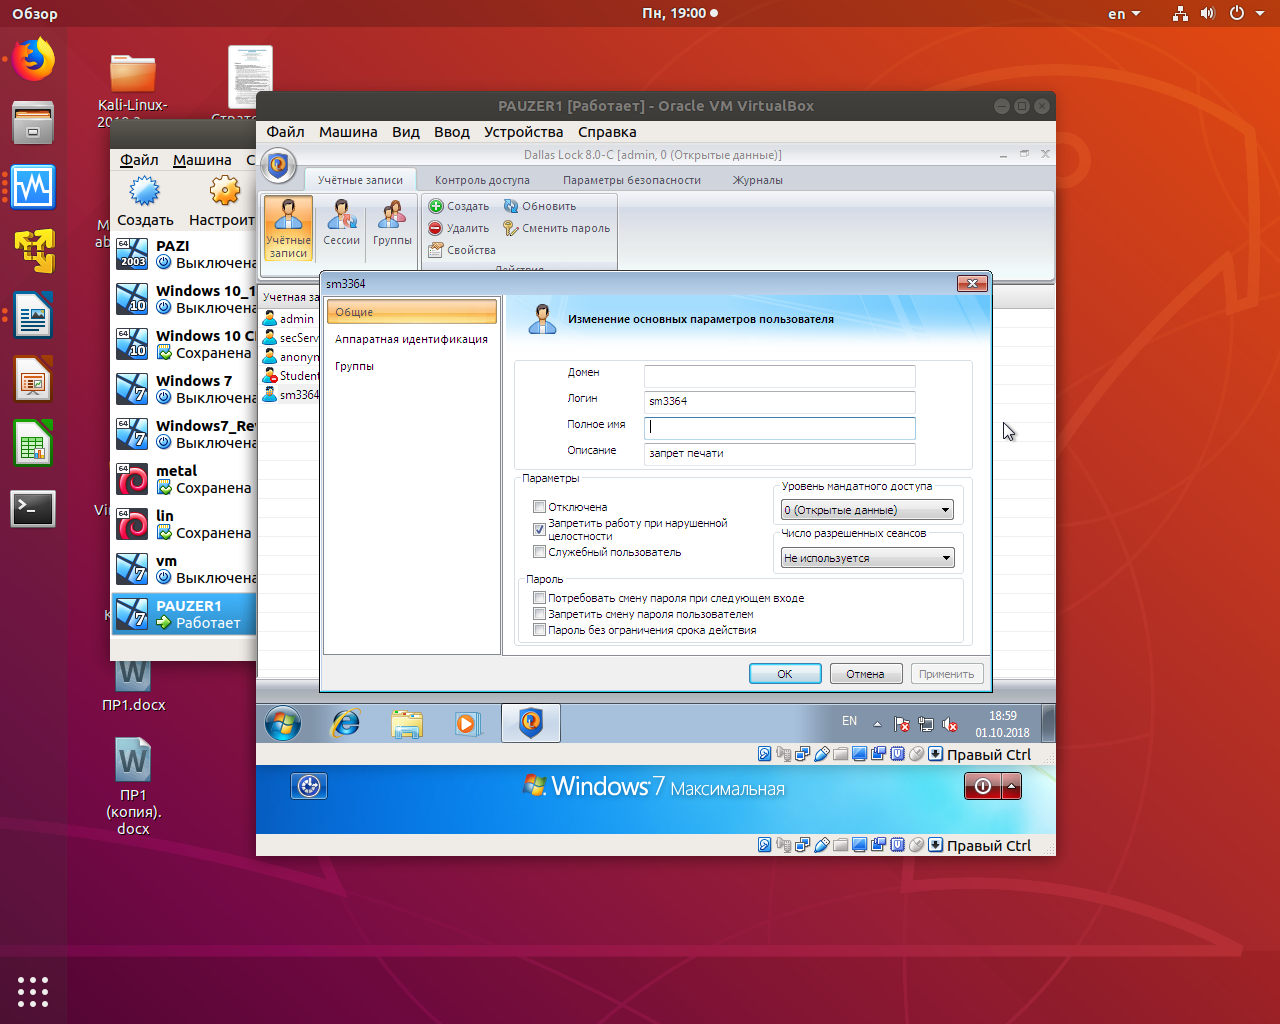
\includegraphics[width=.8\textwidth]{images/3.png}
	\caption{Запрет печати}	
\end{figure}

\begin{figure}[H]
	\centering
	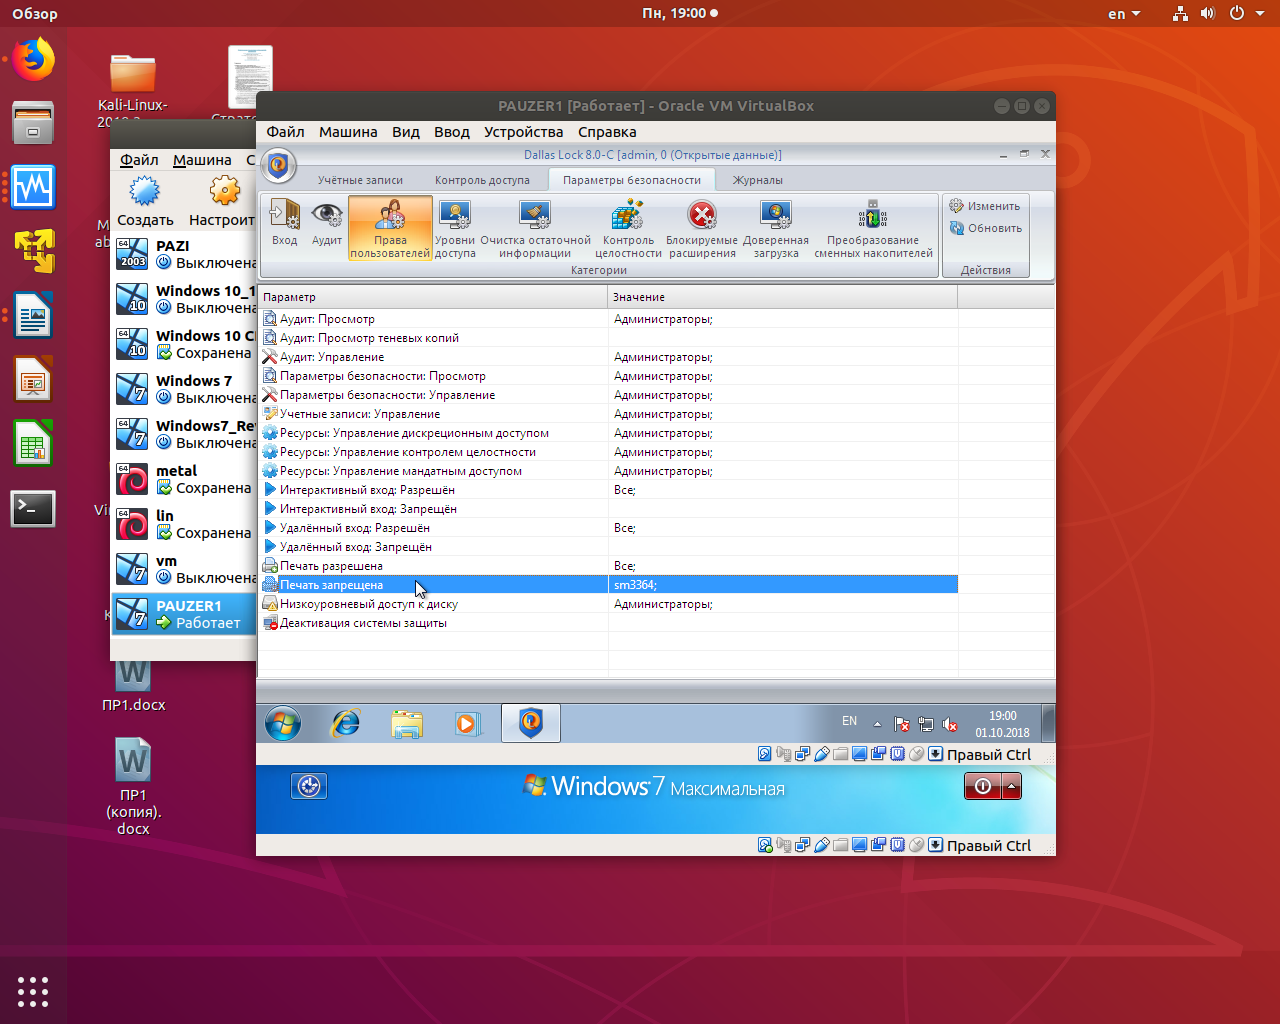
\includegraphics[width=.8\textwidth]{images/4.png}
	\caption{Запрет печати}	
\end{figure}

\begin{figure}[H]
	\centering
	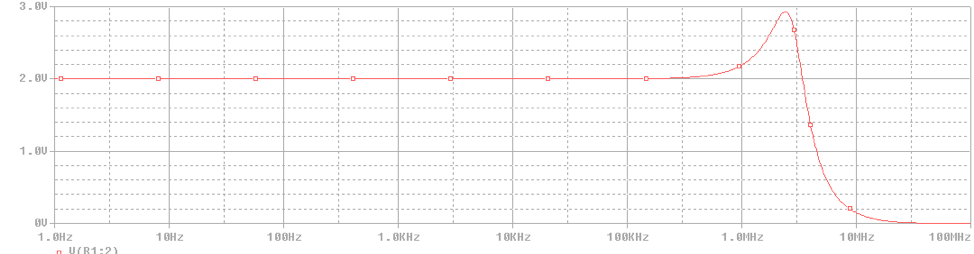
\includegraphics[width=.8\textwidth]{images/5.png}
	\caption{Запрет печати}
\end{figure}

\begin{figure}[H]
	\centering
	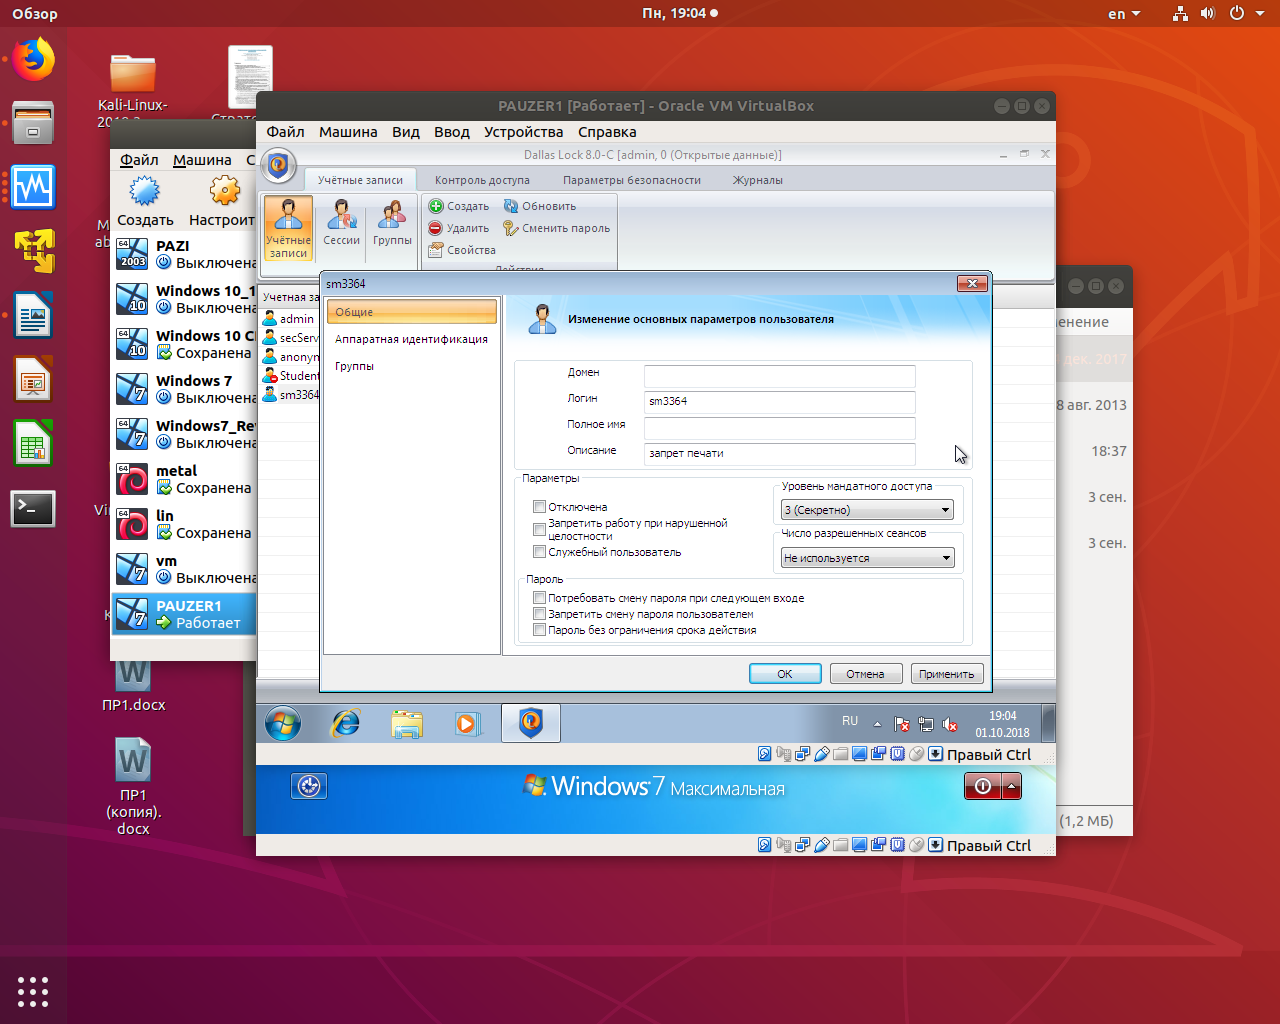
\includegraphics[width=.8\textwidth]{images/6.png}
	\caption{Настройки мандатного доступа}
\end{figure}

\begin{figure}[H]
	\centering
	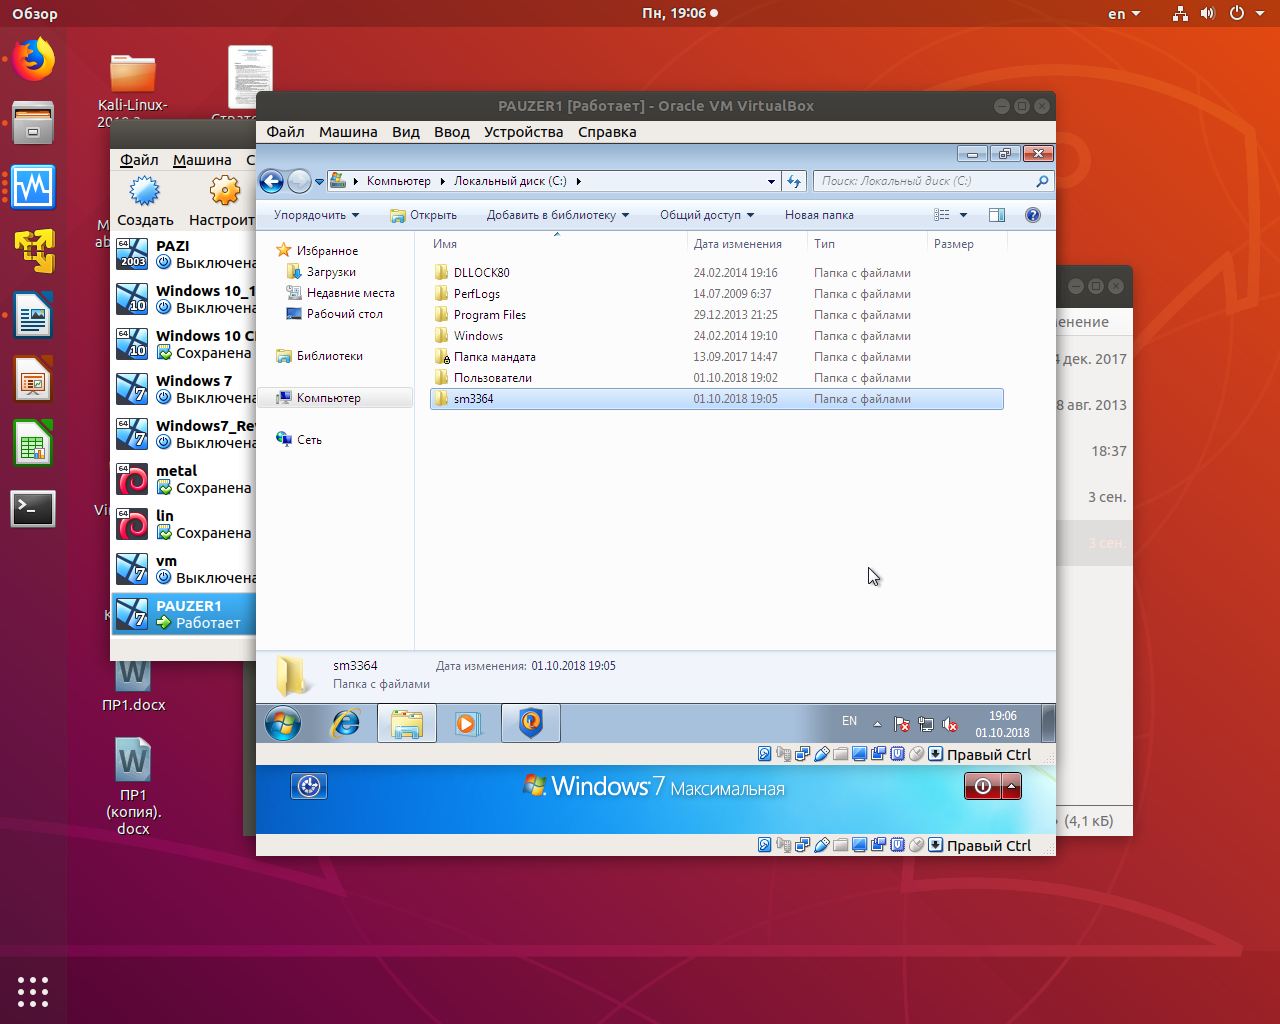
\includegraphics[width=.8\textwidth]{images/7.png}
	\caption{Настройки мандатного доступа}
\end{figure}

\begin{figure}[H]
	\centering
	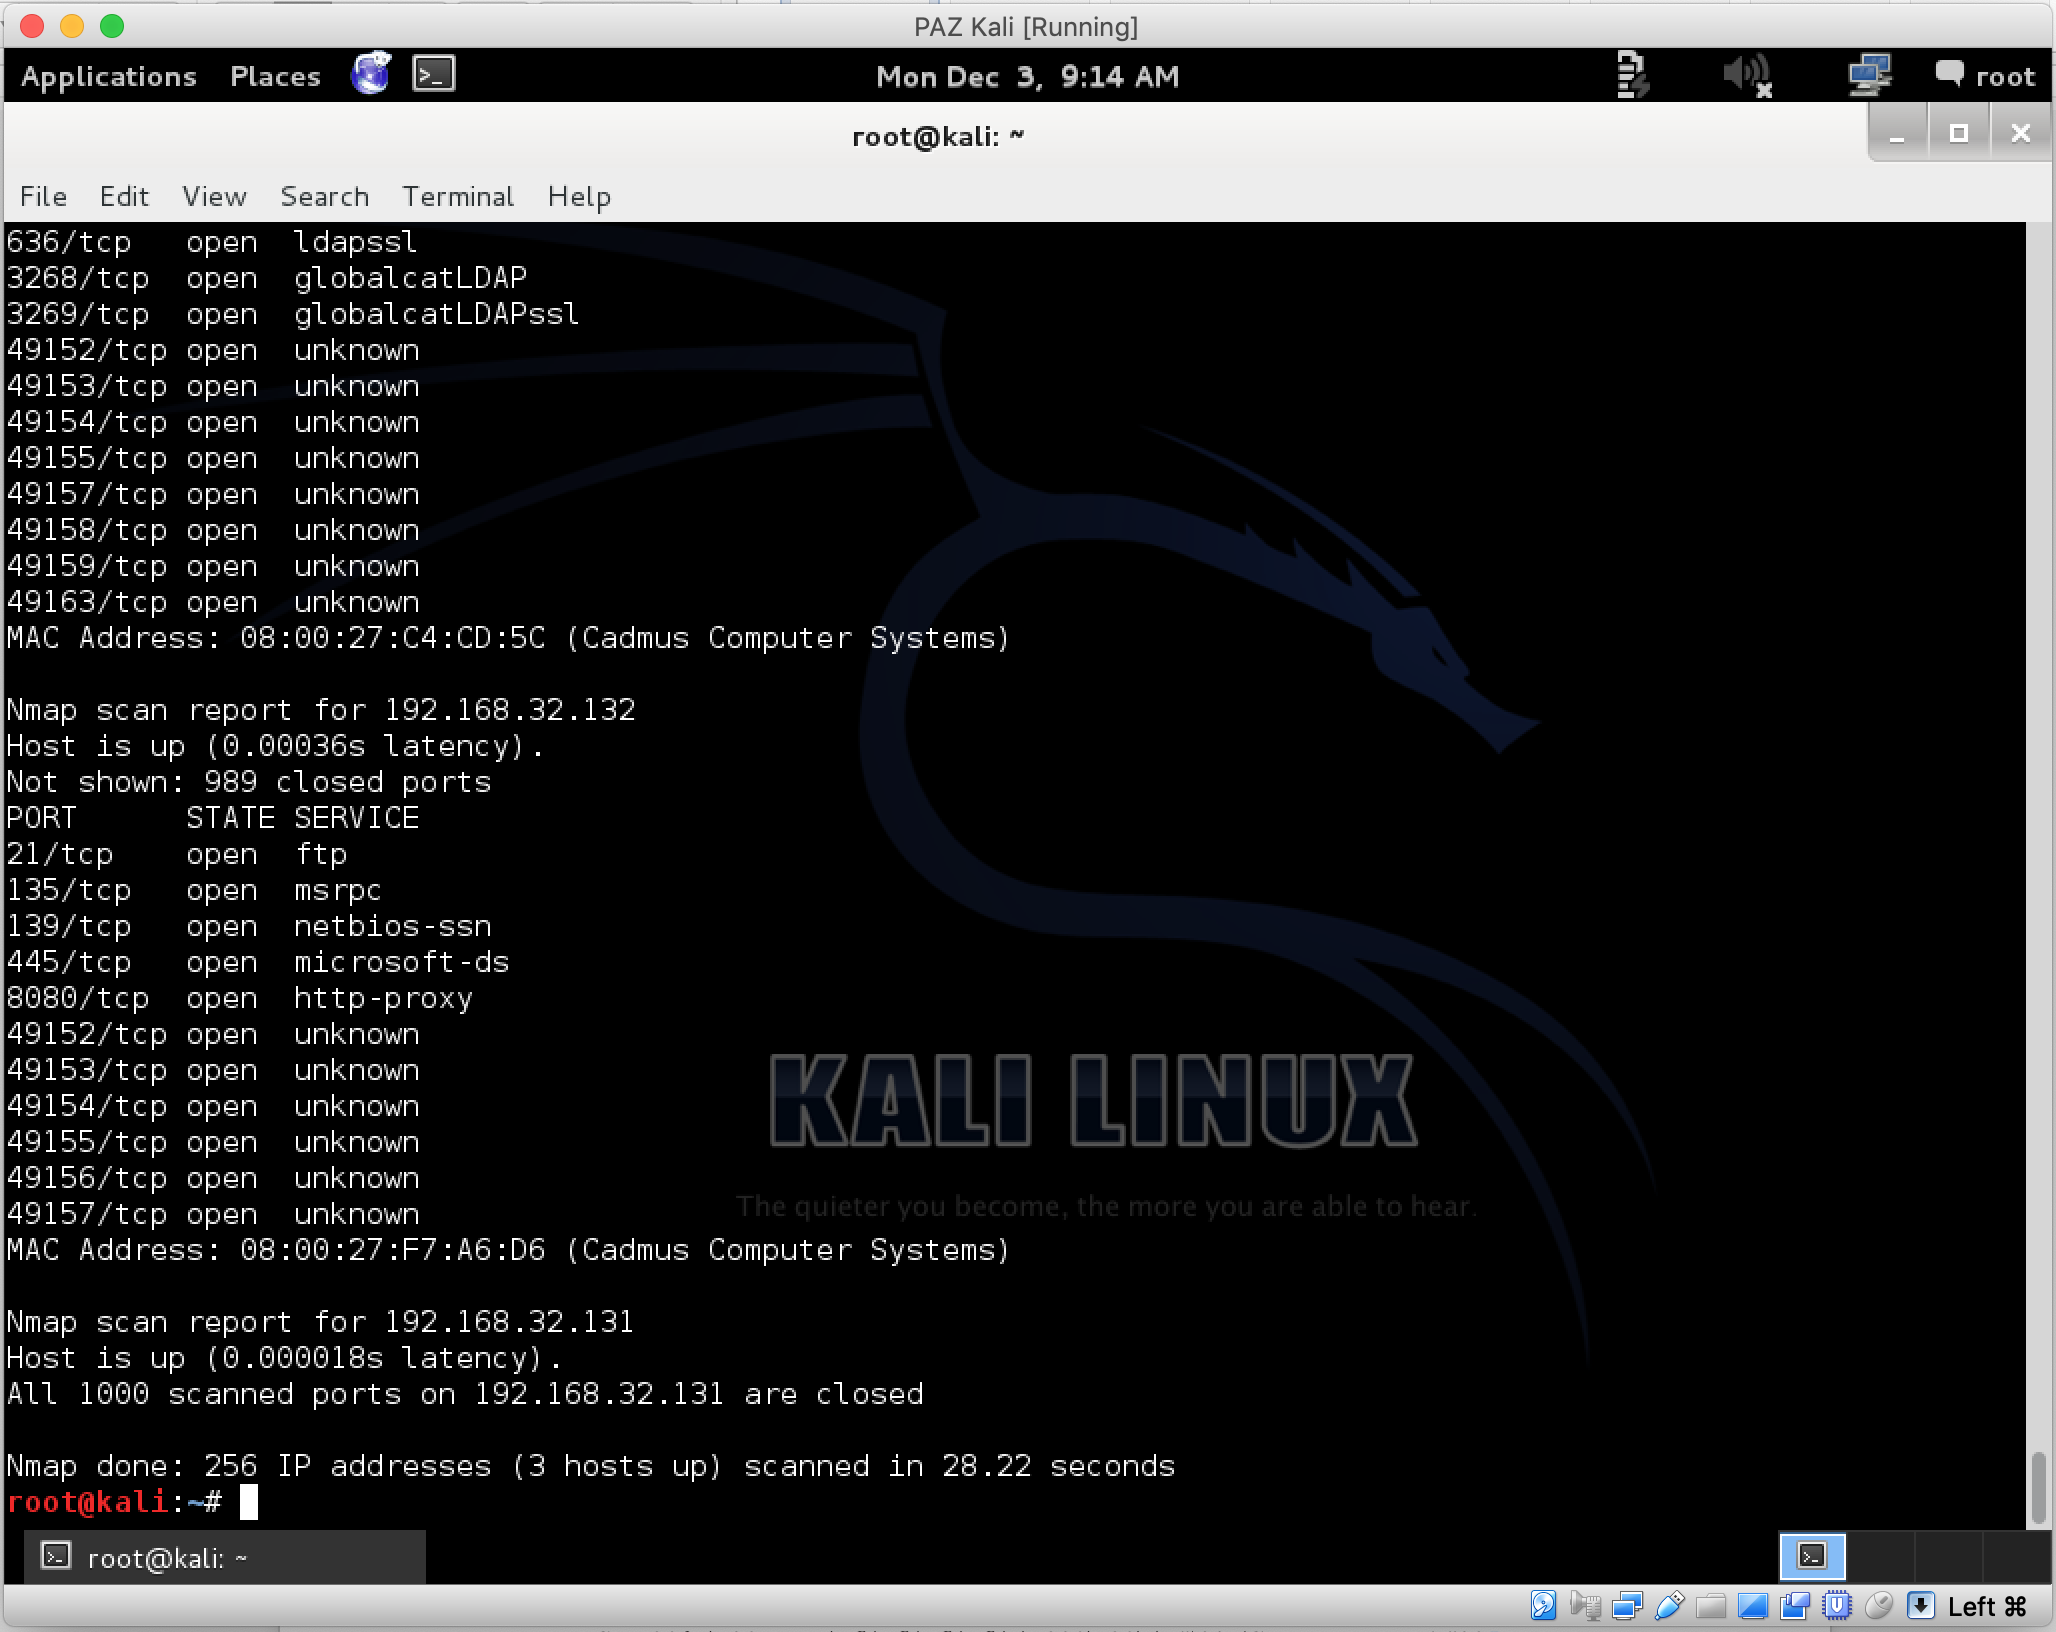
\includegraphics[width=.8\textwidth]{images/8.png}
	\caption{Настройки мандатного доступа}
\end{figure}

\begin{figure}[H]
	\centering
	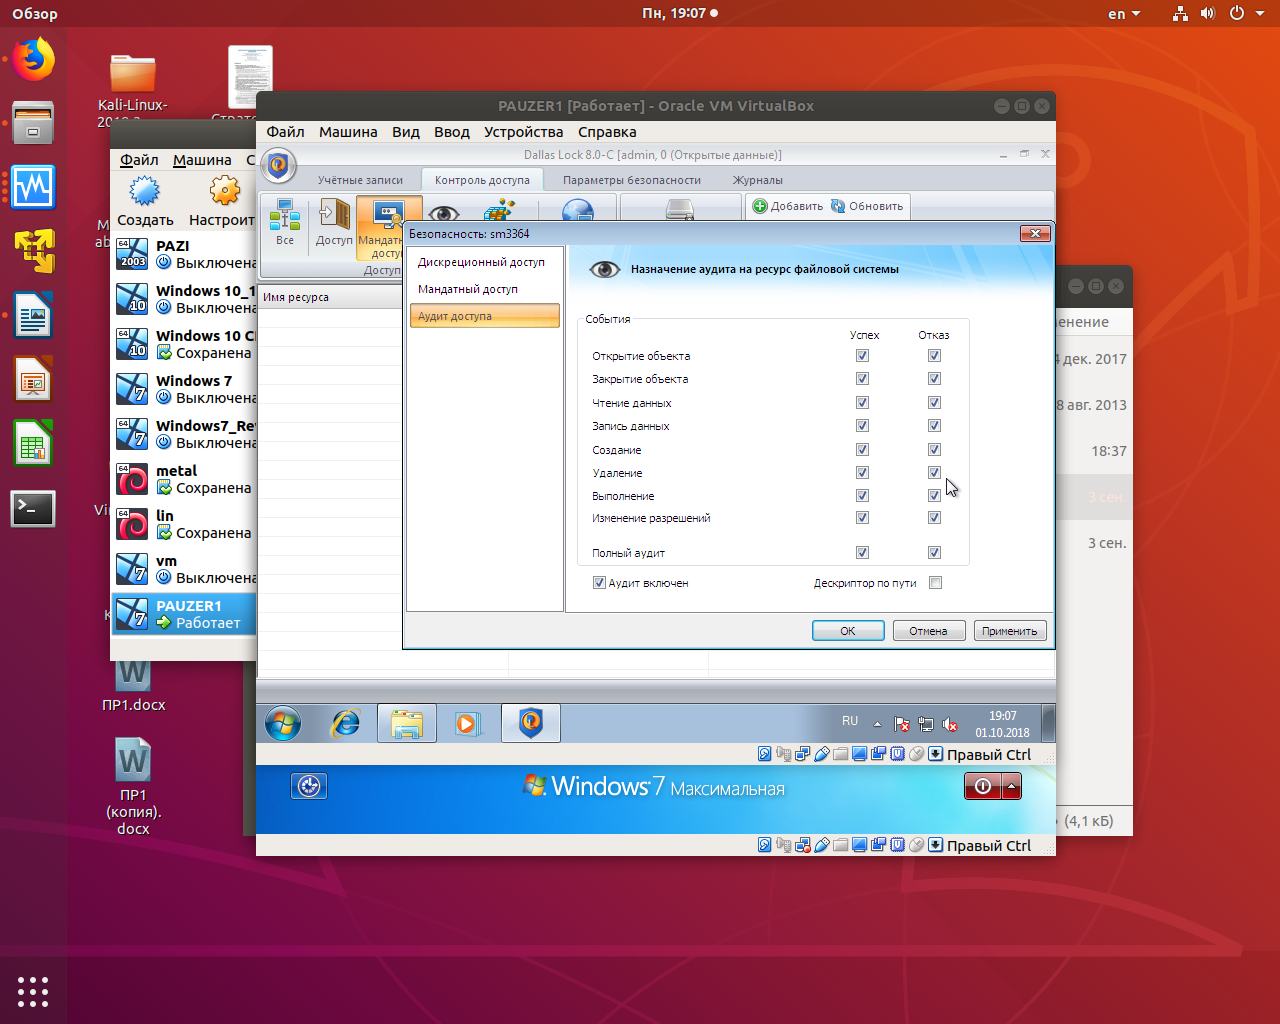
\includegraphics[width=.8\textwidth]{images/9.png}
	\caption{Настройки мандатного доступа}
\end{figure}

\begin{figure}[H]
	\centering
	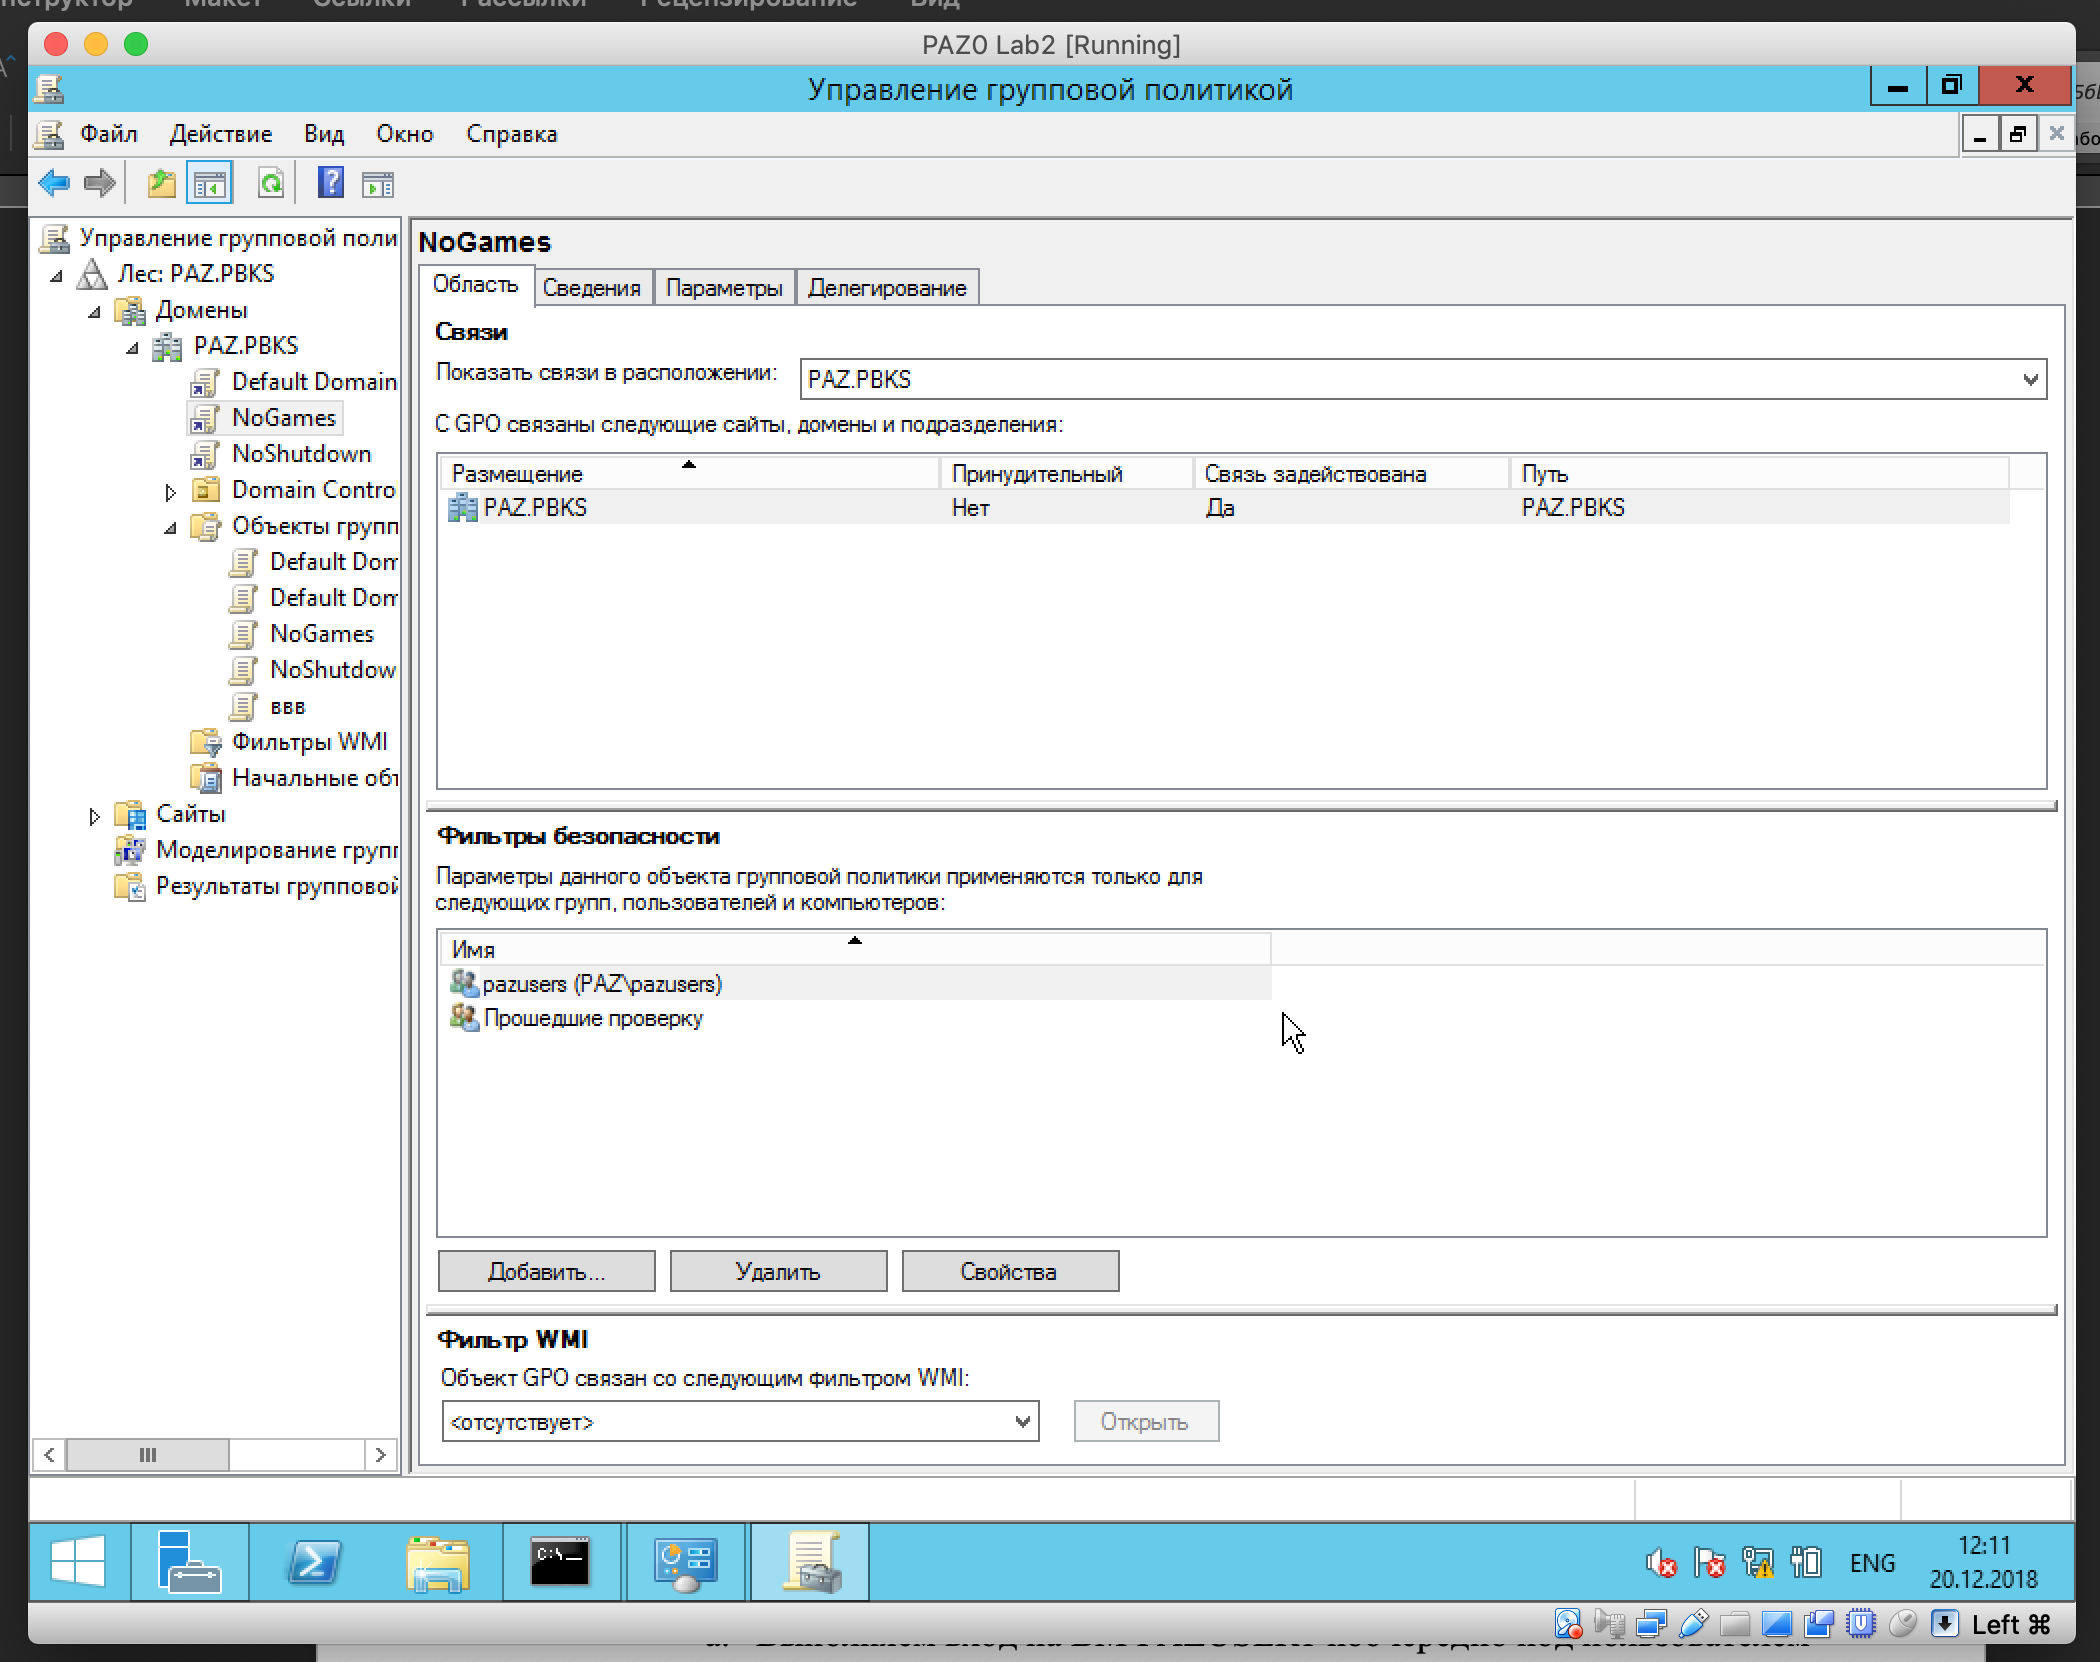
\includegraphics[width=.8\textwidth]{images/10.png}
	\caption{Настройки мандатного доступа}
\end{figure}

\begin{figure}[H]
	\centering
	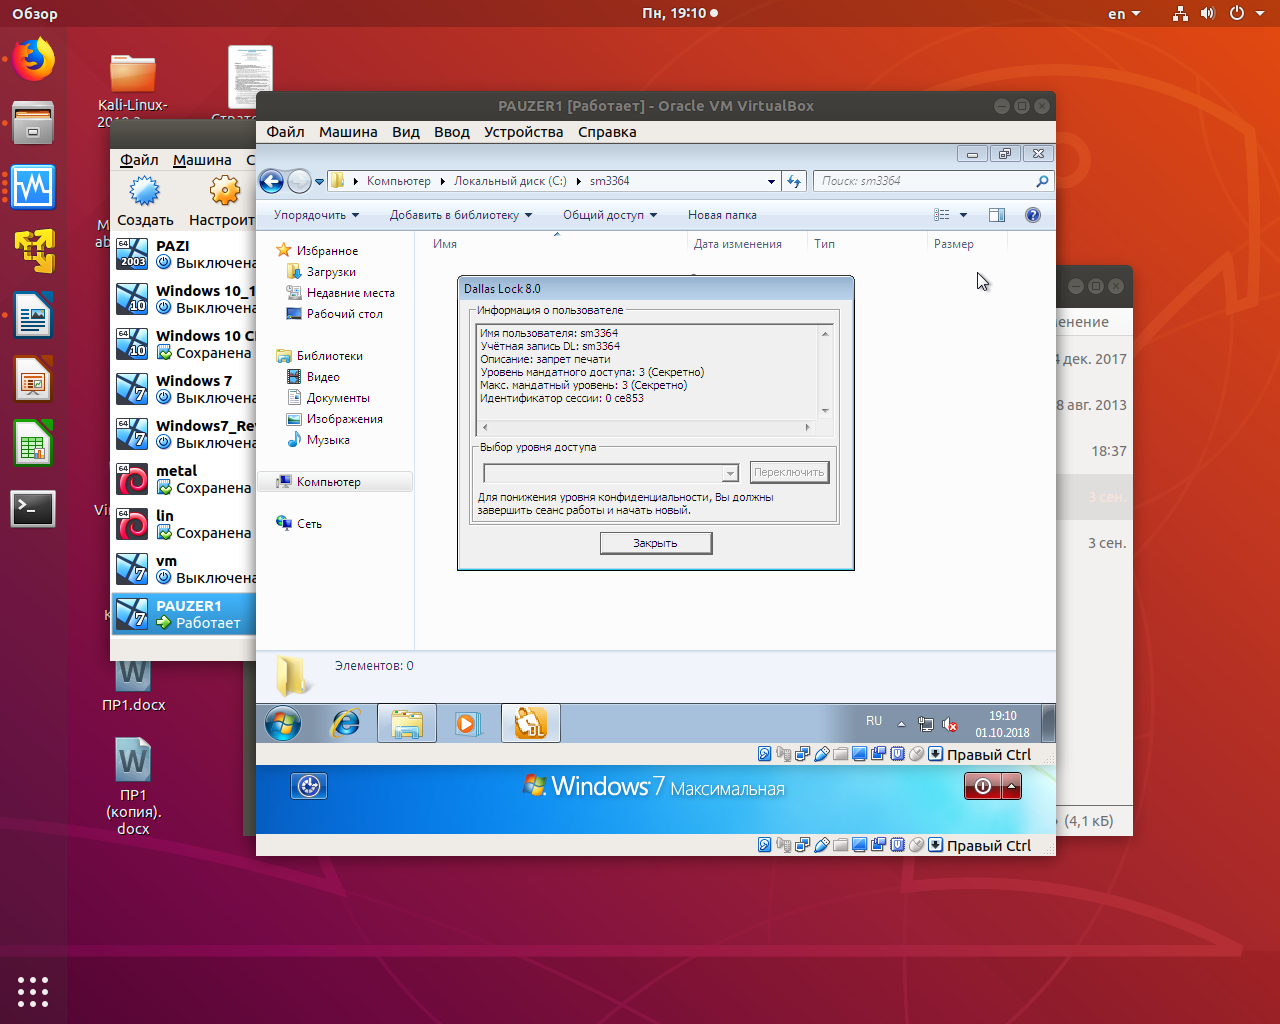
\includegraphics[width=.8\textwidth]{images/11.png}
	\caption{Настройки мандатного доступа}
\end{figure}

\begin{figure}[H]
	\centering
	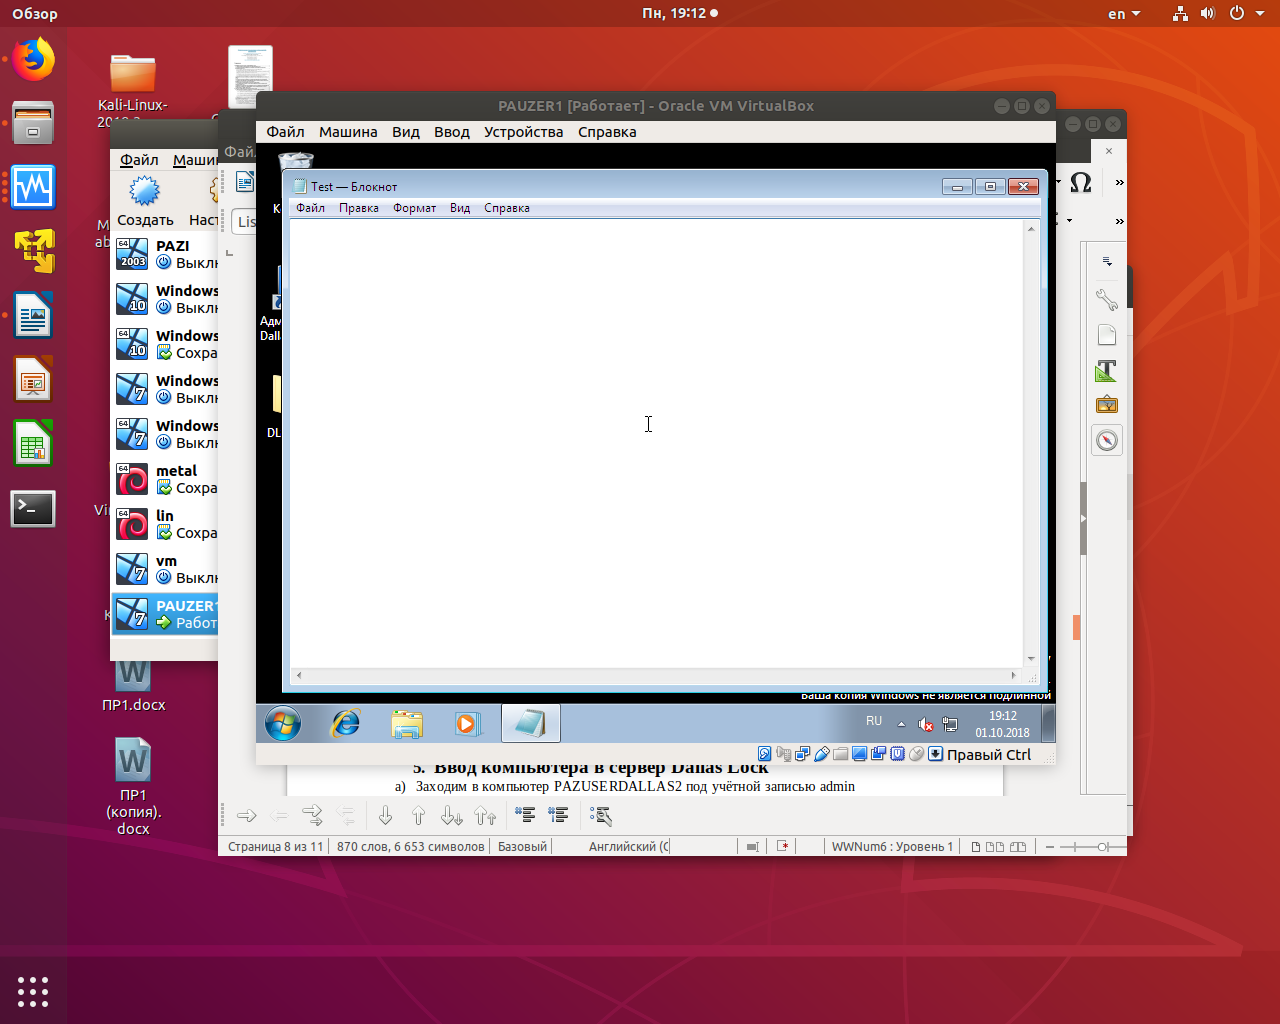
\includegraphics[width=.8\textwidth]{images/12.png}
	\caption{Контроль целостности}
\end{figure}

\begin{figure}[H]
	\centering
	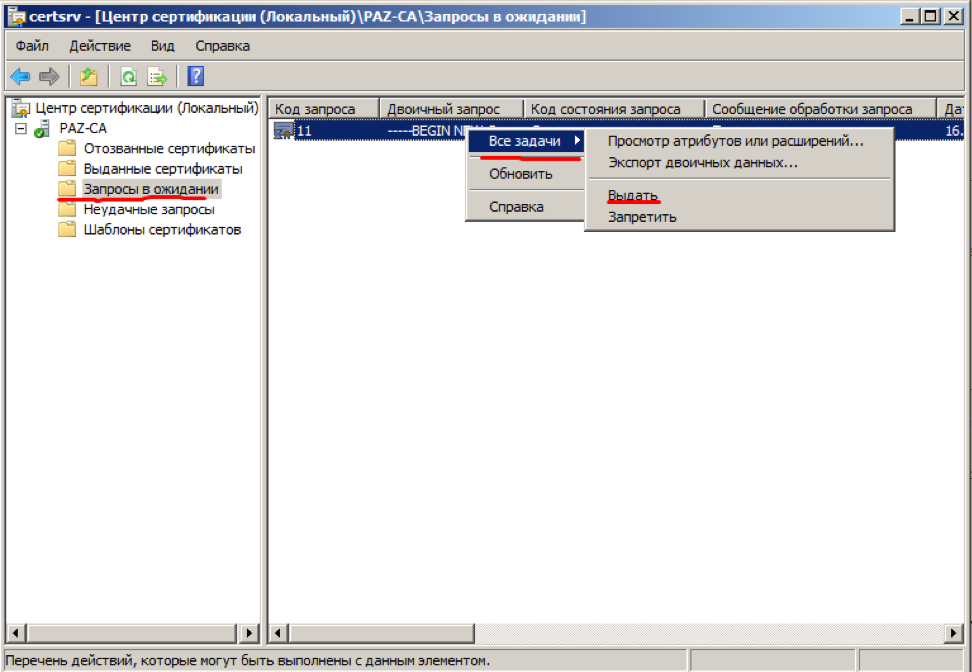
\includegraphics[width=.8\textwidth]{images/13.png}
	\caption{Контроль целостности}
\end{figure}

\begin{figure}[H]
	\centering
	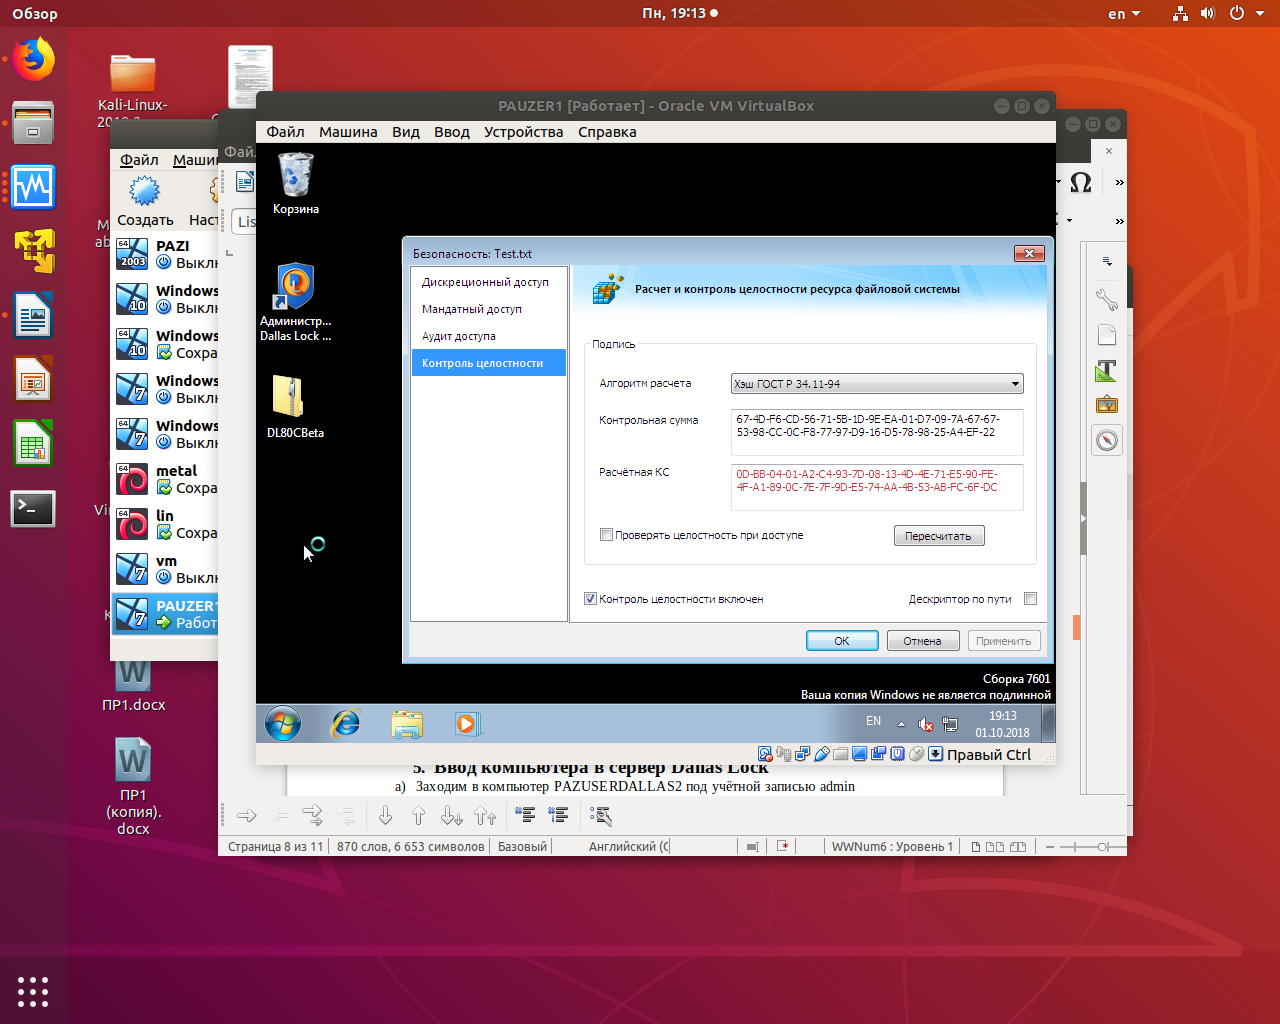
\includegraphics[width=.8\textwidth]{images/14.png}
	\caption{Контроль целостности}
\end{figure}

\begin{figure}[H]
	\centering
	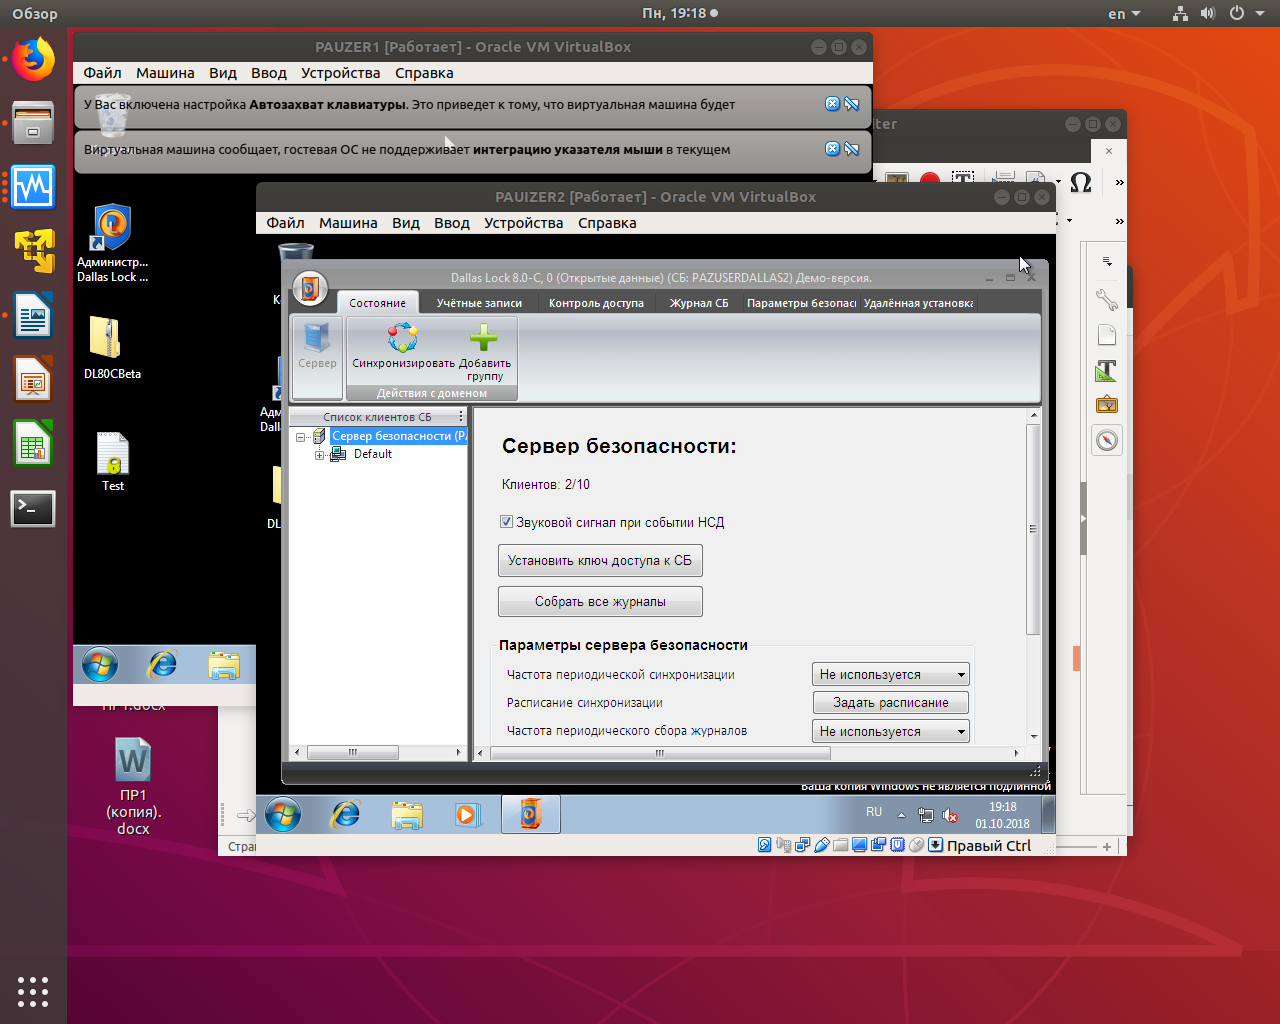
\includegraphics[width=.8\textwidth]{images/15.png}
	\caption{Ввод компьютера в сервер Dallas Lock}
\end{figure}

\begin{figure}[H]
	\centering
	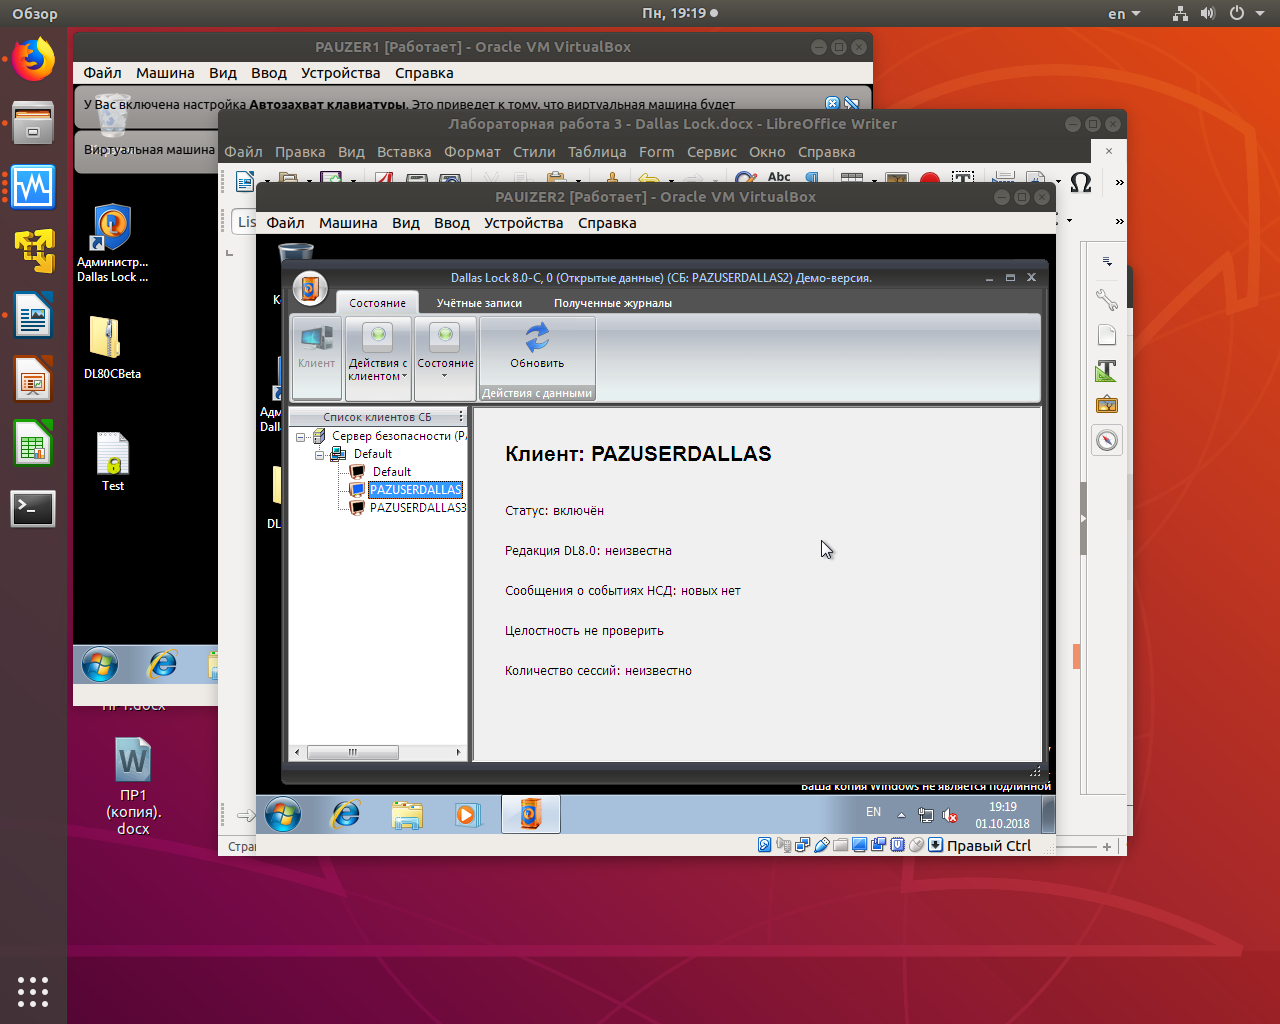
\includegraphics[width=.8\textwidth]{images/16.png}
	\caption{Ввод компьютера в сервер Dallas Lock}
\end{figure}

\begin{figure}[H]
	\centering
	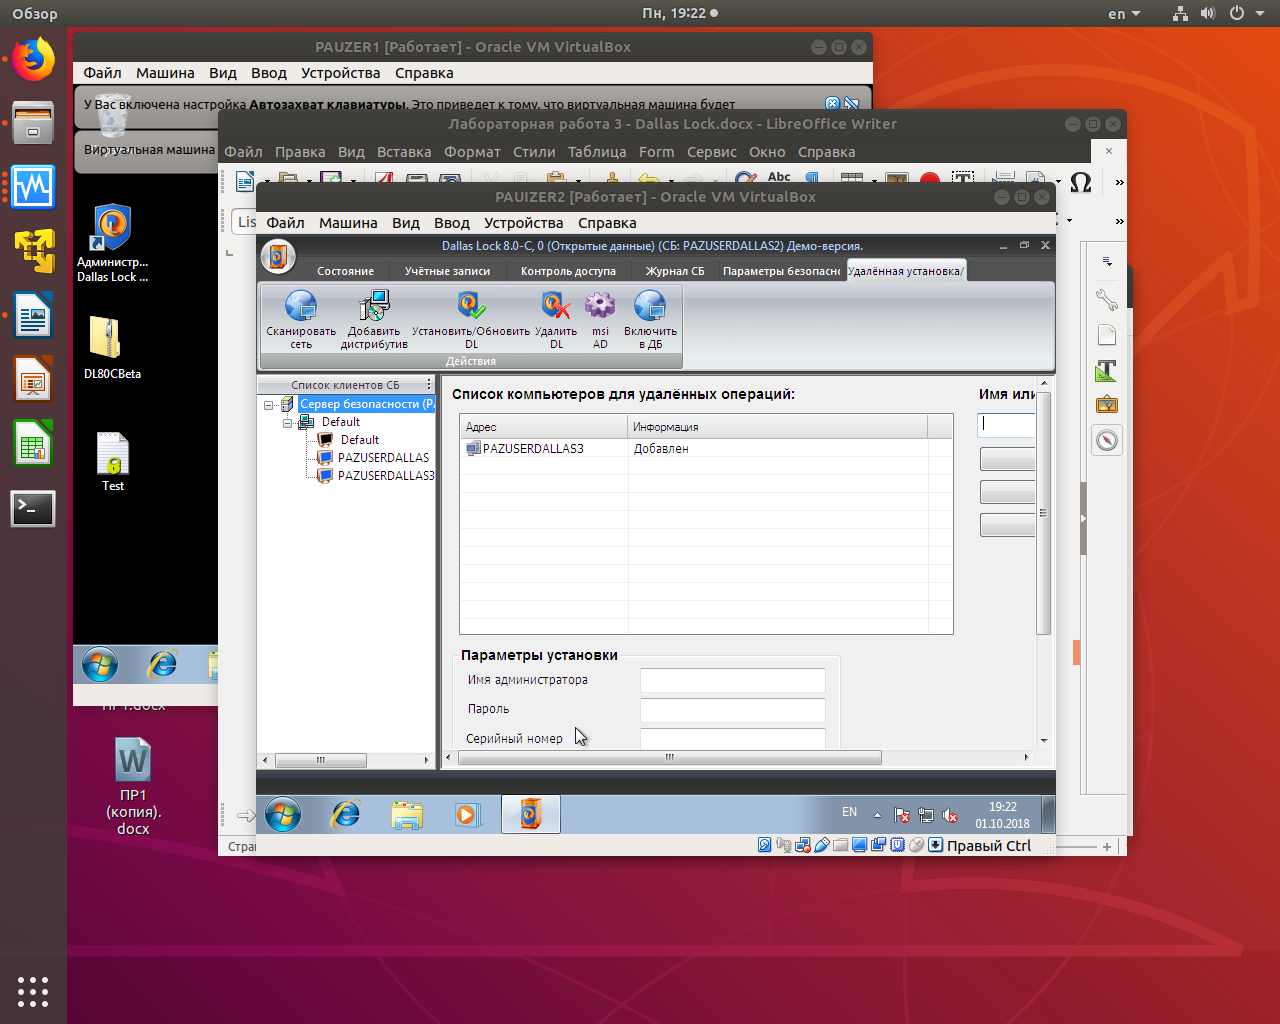
\includegraphics[width=.8\textwidth]{images/17.png}
	\caption{Ввод компьютера в сервер Dallas Lock}
\end{figure}

\begin{figure}[H]
	\centering
	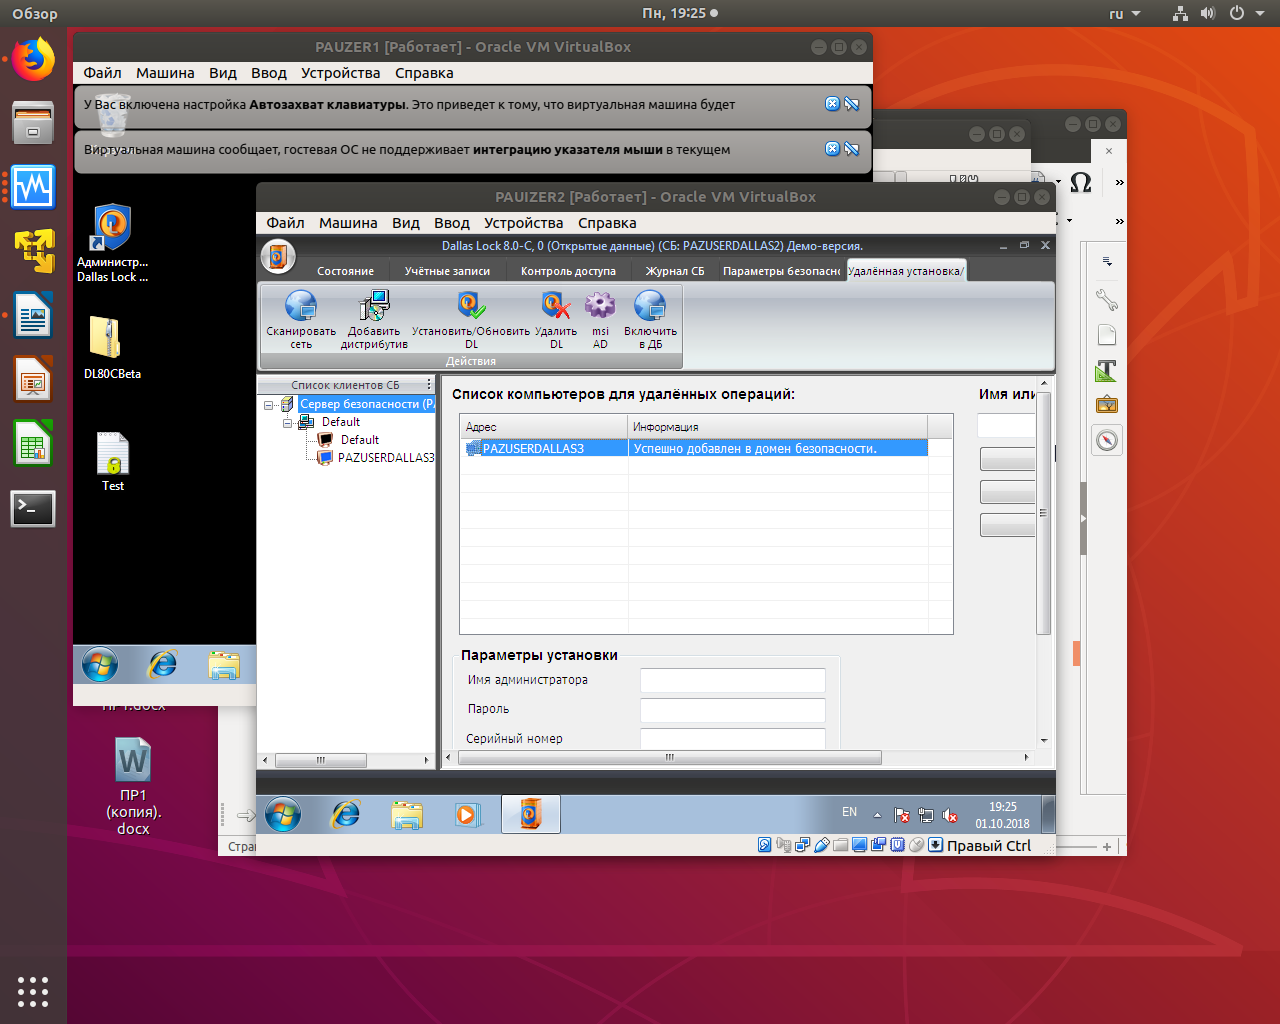
\includegraphics[width=.8\textwidth]{images/18.png}
	\caption{Ввод компьютера в сервер Dallas Lock}
\end{figure}

\begin{figure}[H]
	\centering
	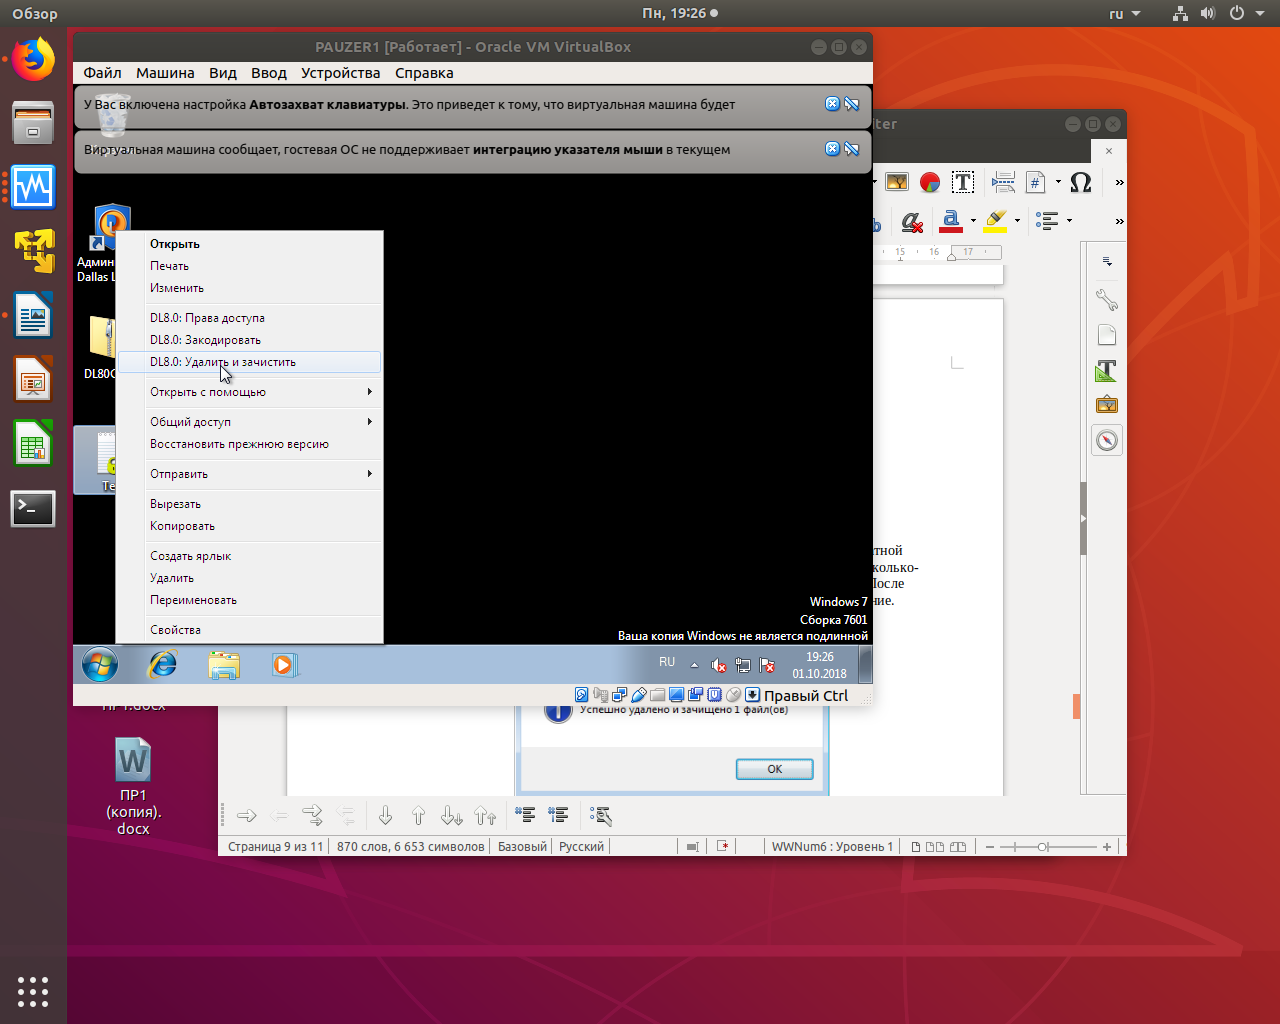
\includegraphics[width=.8\textwidth]{images/19.png}
	\caption{Механизм зачистки остаточной информации}
\end{figure}

\begin{figure}[H]
	\centering
	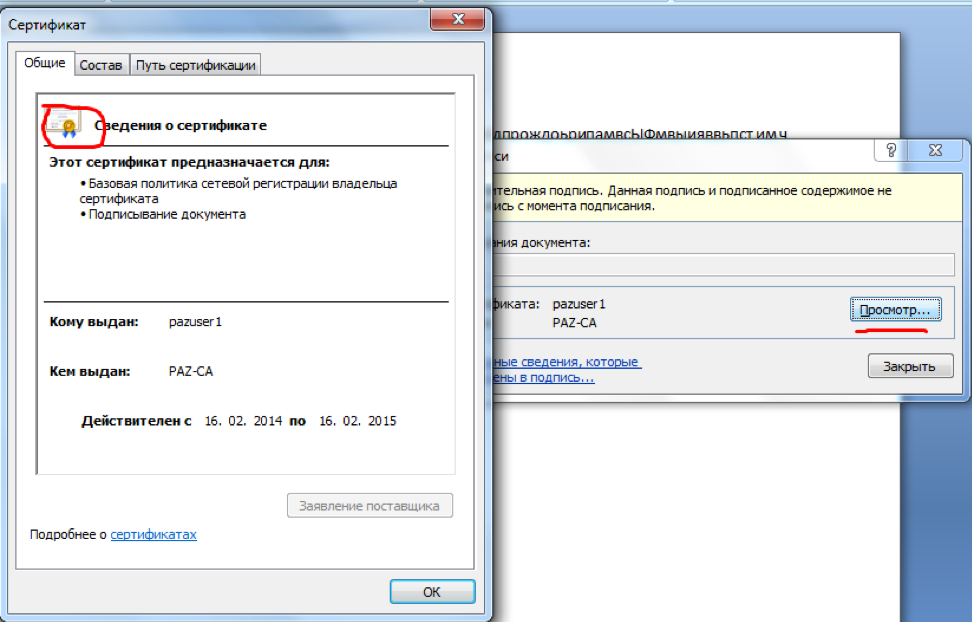
\includegraphics[width=.8\textwidth]{images/20.png}
	\caption{Механизм зачистки остаточной информации}
\end{figure}
